\input{./.econtexRoot}\documentclass[\econtexRoot/SolvingMicroDSOPs]{subfiles}
% econtexRoot gets obliterated by the documentclass command 
%\input{./.econtexRoot}\documentclass[SolvingMicroDSOPs]{subfiles}
\input{./.econtexRoot}\onlyinsubfile{% https://tex.stackexchange.com/questions/463699/proper-reference-numbers-with-subfiles
    \csname @ifpackageloaded\endcsname{xr-hyper}{%
      \externaldocument{\econtexRoot/SolvingMicroDSOPs}% xr-hyper in use; optional argument for url of main.pdf for hyperlinks
    }{%
      \externaldocument{\econtexRoot/SolvingMicroDSOPs}% xr in use
    }%
    \renewcommand\labelprefix{}%
    % Initialize the counters via the labels belonging to the main document:
}



% Get xrefs; only works properly if main file has already been successfully compiled
\onlyinsubfile{\externaldocument{SolvingMicroDSOPs}} 



\begin{document}
\hypertarget{multiple-control-variables}{}
\section{Multiple Control Variables}

We now consider how to solve problems with multiple control variables.  (To reduce notational complexity, in this section we set $\PermGroFac_{\prd}=1~\forall~t$; the time- or age-varying growth factor will return when we consider life cycle problems below).

\subsection{Theory}\label{subsec:MCTheory}
The new control variable that the consumer can now choose is captured by the Greek character called `stigma,' which represents the  share $\Shr$ of their disposable assets to invest in the risky asset (conventionally interpreted as the stock market).  Designating the return factor for the risky asset as $\Risky$ and the share of the portfolio invested in $\Risky$ as $\Shr$, the realized portfolio rate of return $\Rport$ as a function of the share $\Shr$ is:
\begin{equation}\begin{gathered}\begin{aligned}
      \Rport(\Shr) &= \Rfree+(\Risky-\Rfree)\Shr \label{eq:Shr}.
    \end{aligned}\end{gathered}\end{equation}
%\renewcommand{\prd}{t}
% Traditionally, portfolio choice models have been vague about \emph{when} exactly the portfolio optimization problem is solved.
If we imagine the portfolio share decision as being made simultaneously with the ${c}_{\prd}$ decision, a traditional way of writing the problem is (substituting the budget constraint):
\begin{equation}\begin{gathered}\begin{aligned}
      {\vFunc}_{\prd}({m}_{\prd})  & = \max_{\{\cFunc_{\prd},\Shr\}} ~~  \uFunc({c}_{\prd}) +  \ExMidStp[\DiscFac {\vFunc}_{\prd+1}(({m}_{\prd}-{c}_{\prd})\left({\Rfree+(\Risky-\Rfree)\Shr}\right) +        {\TranShkEmp}_{\prd+1})] \label{eq:Bellmanundated}
    \end{aligned}\end{gathered}\end{equation}
where I have deliberately omitted the period-designating subscripts for $\Shr$ and the return factors to highlight the point that, once the consumption and $\Shr$ decisions have been made, it makes no difference to this equation whether we suppose that the risky return factor $\Risky$ is revealed a nanosecond before the end of period $\prd$ or a nanosecond after the beginning of $\prd+1$.

But as a notational choice, there is good reason to designate the realization as happening in $t+1$. A standard way of motivating stochastic returns and wages is to attribute them to ``productivity shocks'' and to assume that the productivity shock associated with a date is the one that affects the production function for that date.

%\renewcommand{\prd}{t} % For the rest of the doc, use generic t vs t+1

\begin{comment}
  Designating the return factor for the risky asset as $\Risky_{\prd+1}$, and using $\Shr_{\prd}$ to represent the proportion of the portfolio invested in this asset before the return is realized after the beginning of $\prd+1$, corresponding to an assumption that the consumer cannot be `net short' and cannot issue net equity), the overall return on the consumer's portfolio between $t$ and $t+1$ will be:
  \begin{verbatimwrite}{./Equations/Rport.tex}
    \begin{equation}\begin{gathered}\begin{aligned}
          \Rport_{\prd+1}  & = \Rfree(1-\Shr_{\prd}) + \Risky_{\prd+1}\Shr_{\prd} \label{eq:return1}
          \\               & = \Rfree + (\Risky_{\prd+1}-\Rfree) \Shr_{\prd} %\label{eq:return2}
        \end{aligned}\end{gathered}\end{equation}
  \end{verbatimwrite}
    \begin{equation}\begin{gathered}\begin{aligned}
        \Rport_{t+1}  & = \Rfree(1-\stigma_{t}) + \Risky_{t+1}\stigma_{t} \label{eq:return1}
        \\               & = \Rfree + (\Risky_{t+1}-\Rfree) \stigma_{t} %\label{eq:return2}
      \end{aligned}\end{gathered}\end{equation}
\unskip
  and the maximization problem is
  \begin{verbatimwrite}{./Equations/PortProb.tex}
    \begin{equation*}\begin{gathered}\begin{aligned}
          {\vFunc}_{\prd}({m}_{\prd})  & = \max_{\{{c}_{\prd},\Shr_{\prd}\}}   ~~ \uFunc({c}_{\prd}) +  \DiscFac
          \ExEndStp[{\vFunc}_{\prd+1}({m}_{\prd+1})]
          \\      & \text{s.t.} \nonumber
          \\      \Rport_{\prd+1}  & = \Rfree + (\Risky_{\prd+1}-\Rfree) \Shr_{\prd}
          \\      {m}_{\prd+1}  & = ({m}_{\prd}-{c}_{\prd})\Rport_{\prd+1} + \TranShkEmp_{\prd+1}
          \\  0       \leq & \Shr_{\prd}  \leq 1, \label{eq:noshorts}
        \end{aligned}\end{gathered}\end{equation*}
  \end{verbatimwrite}
  \begin{eqnarray*}
        {\vFunc}_{t}({m}_{t}) & = & \max_{\{{c}_{t},\varsigma_{t}\}}   ~~ \util({c}_{t}) +  \Discount
        \Ex_{t}[{\vFunc}_{t+1}({m}_{t+1})]
\\      & \text{s.t.} & \nonumber
\\      \Rport_{t+1} & = & \Rfree + (\Risky_{t+1}-\Rfree) \varsigma_{t}
\\      {m}_{t+1} & = & ({m}_{t}-{c}_{t})\Rport_{t+1} + \tShkEmp_{t+1}
\\  0       \leq & \varsigma_{t} & \leq 1, \label{eq:noshorts}
\end{eqnarray*}
\unskip

  The first order condition with respect to ${c}_{\prd}$ is almost identical to that in the single-control problem, equation (\ref{eq:upceqEvtp1}); the only difference is that the nonstochastic interest factor $\Rfree$ is now replaced by the portfolio return ${\Rport}_{\prd+1}$,
  \begin{verbatimwrite}{./Equations/valfuncFOCRtilde.tex}
    \begin{equation}\begin{gathered}\begin{aligned}
          \uFunc^{{c}}({c}_{\prd})  & = \DiscFac \ExEndStp [{\Rport}_{\prd+1} \vFunc^{{m}}_{\prd+1}({m}_{\prd+1})] \label{eq:valfuncFOCRtilde},
        \end{aligned}\end{gathered}\end{equation}
  \end{verbatimwrite}
    \begin{equation}\begin{gathered}\begin{aligned}
        \uFunc^{{c}}({c}_{t})  & = \DiscFac \ExEndStep [{\Rport}_{t+1} \vFunc^{{m}}_{t+1}({m}_{t+1})] \label{eq:valfuncFOCRtilde},
      \end{aligned}\end{gathered}\end{equation}
\unskip
  and the Envelope theorem derivation remains the same,
  yielding the Euler equation for consumption
  \begin{verbatimwrite}{./Equations/EulercRiskyR.tex}
    \begin{equation}\begin{gathered}\begin{aligned}
          \uFunc^{{c}}({c}_{\prd})  & = \ExEndStp[\DiscFac {\Rport}_{\prd+1} \uFunc^{{c}}({c}_{\prd+1})]. \label{eq:EulercRiskyR}
        \end{aligned}\end{gathered}\end{equation}
  \end{verbatimwrite}
    \begin{equation}\begin{gathered}\begin{aligned}
    \util^{\prime}({c}_{t})  & = \Ex_{t}[\Discount {\Rport}_{t+1} \util^{\prime}({c}_{t+1})]. \label{eq:EulercRiskyR}
  \end{aligned}\end{gathered}\end{equation}
\unskip

  The first order condition with respect to the risky portfolio share is
  \begin{verbatimwrite}{./Equations/FOCw.tex}
    \begin{equation}\begin{gathered}\begin{aligned}
          0  & = \ExEndStp[{\vFunc}_{\MidStpNxt}^{{m}}({m}_{\prd+1})(\Risky_{\prd+1}-\Rfree){a}_{\prd}] \notag
          \\         & = \ExEndStp\left[\uFunc^{{c}}\left(\cFunc_{\prd+1}({m}_{\prd+1})\right)(\Risky_{\prd+1}-\Rfree)\right]{a}_{\prd} 
          \\         & = \ExEndStp\left[\uFunc^{{c}}\left(\cFunc_{\prd+1}({m}_{\prd+1})\right)(\Risky_{\prd+1}-\Rfree)\right], \label{eq:FOCw}        
        \end{aligned}\end{gathered}\end{equation}
  \end{verbatimwrite}
    \begin{equation}\begin{gathered}\begin{aligned}
    0  & = \Ex_{t}[{\vFunc}_{t+1}^{\prime}({m}_{t+1})(\Risky_{t+1}-\Rfree){a}_{t}] \notag
    \\         & = {a}_{t}\Ex_{t}\left[\util^{\prime}\left(\cFunc_{t+1}({m}_{t+1})\right)(\Risky_{t+1}-\Rfree)\right] \label{eq:FOCw}.
  \end{aligned}\end{gathered}\end{equation}
\unskip
  where the last line follows because $0/a_{\prd}=0$.

  As before, we define $\vEnd$ as a function that yields the expected $t+1$ value of ending period $t$ with assets ${a}_{\prd}$.  However, now that there are two control variables, the expectation must be defined as a function of the chosen values of both of those variables, because expected end-of-period value will depend not just on how much the agent saves, but also on how the saved assets are allocated between the risky and riskless assets.  Thus we define
  \begin{equation*}\begin{gathered}\begin{aligned}
        \vMid({a}_{\prd},\Shr_{\prd})  & = \DiscFac {\vFunc}_{\arvlstepShr}({m}_{\prd+1})
      \end{aligned}\end{gathered}\end{equation*}
  which has derivatives
  \begin{equation}\begin{gathered}\begin{aligned}
        \vMid^{{a}}  & = \ExEndStp[\DiscFac {\Rport}_{\prd+1}{\vFunc}_{\prd+1}^{m}({m}_{\prd+1})] = \ExEndStp[\DiscFac {\Rport}_{\prd+1}{\uFunc}_{\prd+1}^{{c}}(\cFunc_{\prd+1}({m}_{\prd+1}))]
      \end{aligned}\end{gathered}\end{equation}
  \begin{equation}\begin{gathered}\begin{aligned}
        \vMid^{\Shr}  & = \ExEndStp[\DiscFac (\Risky_{\prd+1}-\Rfree){\vFunc}_{\prd+1}^{m}({m}_{\prd+1})  ]a_{\prd} = \ExEndStp[\DiscFac (\Risky_{\prd+1}-\Rfree){\uFunc}_{\prd+1}^{{c}}(\cFunc_{\prd+1}({m}_{\prd+1}))  ]a_{\prd} \notag
      \end{aligned}\end{gathered}\end{equation}
  implying that the first order conditions (\ref{eq:EulercRiskyR}) and
  (\ref{eq:FOCw}) can be rewritten
  \begin{equation}\begin{gathered}\begin{aligned}
        \uFunc^{{c}}({c}_{\prd})  & = \vMid^{{a}}({m}_{\prd}-{c}_{\prd},\Shr_{\prd}) \label{eq:FOCc}
      \end{aligned}\end{gathered}\end{equation}
  and 
  \begin{equation}\begin{gathered}\begin{aligned}
        0  & = \vFunc^{\Shr}_{\vMidStgShr}({a}_{\prd},\Shr_{\prd}). \label{eq:FOCShr}
      \end{aligned}\end{gathered}\end{equation}
\end{comment}

\hypertarget{stages-within-a-period}{}
\subsection{Stages Within a Period}\label{subsec:stageswithin}


Solving simultaneously for the two variables $\Shr$ and ${c}$ can be computationally challenging.  Fortunately, there is a simple solution: Break the problem into two `stages.'\footnote{cite mnw and ael papers.}

As demonstrated in \eqref{eq:Bellmanundated}, the mathematical solution for the optimal portfolio share is the same whether we conceive the shocks as occuring at the end of $\prd$ or the beginning of $\prd+1.$  But our tripartite dissection of the problem above into $\{\prd_{\BegMark},\prd,\prd_{\EndMark}\}$ steps was motivated partly by a desire to invent a notation that can allow for construction of standalone `stages' whose only connection to the subsequent problem is through the continuation-vaue function.

To illustrate this point, consider the standalone problem of an `investor' whose continuation value function $\vFunc_{[\Shr]_\cntn}$ depends only on the amount of liquid assets $\lqdcntn$ with which they end up after the realization of the stochastic $\Risky$ return.  The expected value that the investor will obtain from any combination of initial $\lqd_{\arvl}$ and $\Shr$ is the expectation of the continuation value function over the liquid assets that result from the portfolio choice:
\begin{equation}\begin{gathered}\begin{aligned}
      \vFunc_{[\Shr]}({\lqdarvl})
      = & \max_{\Shr}~ \Ex\left[        \vFunc_{[\Shr]_{_\cntn}}\left(\Rport(\Shr){\lqdarvl}        \right)
      \right] \label{eq:vMidStgShr}
    \end{aligned}\end{gathered}\end{equation}
where we have omitted any designator like $\prd$ for the period in which this problem is solved because, with the continuation value function defined already as $\vEnd({\lqd}_{_\cntn})$, the problem is self-contained -- it need make no reference to events later or earlier than its own moment, defined as the interval within which risky returns are realized.  The solution to this problem will yield an optimal $\Shr$ decision rule $\optml{\Shr}(\lqd_{_\arvl}).$  Finally, we can specify the value of an investor `arriving' with $\lqdarvl$ as the expected value that will be obtained when the investor invests optimally, generating the (optimally) stochastic portfolio return factor $\optml{\Rport}(\lqdarvl)=\Rport(\optml{\Shr}(\lqdarvl))$:
\begin{equation}\begin{gathered}\begin{aligned}
      \vFunc_{\arvl}({\lqdarvl})  = & \Ex[\vFunc_{[\Shr]_{_\cntn}}(\overbrace{
        \optml{\Rport}(\lqdarvl){\lqdarvl}}^{\lqdcntn})].
    \end{aligned}\end{gathered}\end{equation}

The reward for all our painful notational investment is that it is now clear that \emph{exactly the same code} for solving the portfolio share problem can be used in two distinct models: One in which the $\Risky$ shocks are realized just after the beginning of $\prd$ and one in which they are realized just before the end. In the first case, the `incoming' amount of liquid assets $\lqdarvl$ corresponds to the capital $k_{\prd}$ with which the agent enters the period while the exiting amount of assets corresponds to $b_{\prd}$ (before-labor-income resources) as in \eqref{eq:vNormed} (with the substitution of the $\optml{\Rport}$ for $\RNrm$).  The second case is only a tiny bit trickier: Our assumption that the return shocks happen at the end of $\prd$ means that the problem needs to be altered slightly to bring the steps involving the realization of risky returns fully into period $\prd$; the variable with which the agent ends the period is now ${b}_{\prd}$ and to avoid confusion with the prior model in which we assumed ${k}_{\prd+1}={a}_{\prd}$ we will now define $\kappa_{\prd+1}={b}_{\prd}$.  The continuation value function now becomes
\begin{equation}\begin{gathered}\begin{aligned}
      \vFunc_{\prd_\cntn}({{b}}_{\prd}) & = \DiscFac \vFunc_{_\arvl(\prd+1)}({\kappa}_{\prd+1})
    \end{aligned}\end{gathered}\end{equation}
while the dynamic budget constraint for ${m}$ changes to
\begin{equation}\begin{gathered}\begin{aligned}
      {m}_{\prd} & = {\kappa}_{\prd}+\TranShkEmp_{\prd}
    \end{aligned}\end{gathered}\end{equation}
and the problem in the decision step is now
\begin{equation}\begin{gathered}\begin{aligned}
      \vFunc_{\prd}({m}_{\prd}) & = \max_{{c}}~~\uFunc({c})+\Ex_{\prd}[\vFunc_{\prd_\cntn}({m}_{\prd}-{{c}})]
    \end{aligned}\end{gathered}\end{equation}
while value in the arrival step is now
\begin{equation}\begin{gathered}\begin{aligned}
      \vFunc_{_\arvl\prd}({\kappa}_{\prd}) & = \Ex_{_\arvl\prd}[\vFunc_{\prd}({m}_{\prd})]
    \end{aligned}\end{gathered}\end{equation}
which, \textit{mutatis mutandis}, is the same as in \eqref{eq:vNormed}.

The upshot is that all we need to do is change some of the transition equations and we can use the same code (both for the $\Shr$-stage and the ${c}$-stage) to solve the problem with either assumption about the timing of portfolio choice.  There is even an obvious notation for the two problems: $\vFunc_{_\arvl\prd[\Shr{c}]}$ can be the arrival (beginning-of-period) value function for the version where the portfolio share is chosen at the beginning of the period, and $\vFunc_{_\arvl\prd[{c}\Shr]}$ is initial value for the the problem where the share choice is at the end.




% The second stage in the period will be the solution to the problem of a consumer solving an optimal portfolio choice problem before having made their consumption decision.

% We continue to assume that the consumer enters period $t$ with the single state variable, $k_{\prd}.$  But (as before) the assumption is that this is before the $t$-dated shocks have been realized.  It is at this stage that the consumer makes their portfolio choice, knowing the degree of riskiness of the rate of return but not its period-$t$ realization.  Designating the `share-choice' stage by the control variable $\Shr$ which is the proportion of the portfolio to invest in the risky asset, %the problem's FOC in the new notation is (compare to  \eqref{eq:FOCShr}):

% It will be convenient to designate a stage within a period by naming a given stage in period $\prd$ after the control variable chosen in the middle step of the stage; in this case $\prd[\Shr]$.  The consumer's problem at the $\Shr$ stage is
% \begin{equation}\begin{gathered}\begin{aligned}
%       \vFunc_{\arvlstepShr}({a}_{\prd})  & = \max_{\Shr}~\vMidStgShr({a}_{\prd},\Shr_{\prd}) \label{eq:vMidStgShr}
%     \end{aligned}\end{gathered}\end{equation}
% whose FOC in the new notation is (compare to  \eqref{eq:FOCShr}):
% \begin{equation}\begin{gathered}\begin{aligned}
%       0  & = \vShrMid({a}_{\prd},\Shr_{\prd}). \label{eq:vShrEnd}
%     \end{aligned}\end{gathered}\end{equation}
While the investor's problem cannot be solved using the endogenous gridpoints method,\footnote{Because $\vShrEnd$ is not invertible with respect to $\Shr$, see [references to MNW and AEL's work].} we can solve it numerically for the optimal $\Shr$ at a vector of $\vctr{a}$ ({\aVecCode} in the code)  and then construct an approximated optimal portfolio share function $\Aprx{\optml{\Shr}}(a)$ as the interpolating function among the members of the $\{\vctr{a},\vctr{\Shr}\}$ mapping.  Having done this, we can now calculate a vector of values that correspond to $\aVec$
\begin{equation}\begin{gathered}\begin{aligned}
      \vctr{{v}}_{_\cntn}  & = \vEnd(\vctr{a},\Aprx{\optml{\Shr}}(\vctr{a})), \label{eq:vShrEnd}
    \end{aligned}\end{gathered}\end{equation}
which can be evaluated at the same vector of points $\vctr{a}$ at which $\vctr{\Shr}$ was calculated, generating the vector $\vctr{{v}}_{[\Shr]{_\cntn}}$ whose inverse can again be approximated as above (along with approximations of marginal value, marginal marginal value, etc).% using the interpolating function among points of the $\{\vctr{a},\vVecShr\}$ (and the same can be done to generate an approximation to the marginal value function $\vFunc_{\BegStp}^{\Shr}({a})$, the marginal marginal value function, and so on).

The beauty of this procedure is that, with the approximation to $\vBegStgShr^{a}(a)$ in hand, we can construct our approximation to the consumption function using \emph{exactly the same EGM procedure} that we used in solving the problem \emph{without} a portfolio choice (see \eqref{eq:cGoth}):
\begin{equation}\begin{gathered}\begin{aligned}
      \vctr{c}  & \equiv  \left(\vFunc^{a}_{\prd_\cntn}(\vctr{a})\right)^{-1/\CRRA} \label{eq:cVecPort},
    \end{aligned}\end{gathered}\end{equation}
which, following a procedure identical to that in the EGM subsection \ref{subsec:egm}, yields an approximated consumption function $\Aprx{\cFunc}_{\prd}({m})$.  Thus, again, we can construct the consumption function at nearly zero cost (once we have calculated $\vctr{v}^{a}$).

\subsection{Application}\label{subsec:MCApplication}

In specifying the stochastic process for $\Risky_{\prd+1}$, we follow the common practice of assuming that returns are lognormally distributed, $\log \Risky \sim \mathcal{N}(\eprem+\rfree-\sigma^{2}_{\risky}/2,\sigma^{2}_{\risky})$ where $\eprem$ is the equity premium over the thin returns $\rfree$ available on the riskless asset.\footnote{This guarantees that $\Ex[\Risky] = \EPrem$ is invariant to the choice of $\sigma^{2}_{\eprem}$; see \handoutM{LogELogNorm}.}

As with labor income uncertainty, it is necessary to discretize the rate-of-return risk in order to have a problem that is soluble in a reasonable amount of time.  We follow the same procedure as for labor income uncertainty, generating a set of $n_{\risky}$ equiprobable shocks to the rate of return; in a slight abuse of notation, we will designate the portfolio-weighted return (contingent on the chosen portfolio share in equity, and potentially contingent on any other aspect of the consumer's problem) simply as $\Rport_{i,j}$ (where dependence on $i$ is allowed to permit the possibility of nonzero correlation between the return on the risky asset and the $\TranShkEmp$ shock to labor income (for example, in recessions the stock market falls and labor income also declines).


The direct expressions for the derivatives of $\vEnd$ are
\begin{equation}\begin{gathered}\begin{aligned}
      \vEnd^{{a}}({a}_{\prd},\Shr_{\prd})  & = \DiscFac \left(\frac{1}{n_{\risky} n_{\TranShkEmp}}\right)\sum_{i=1}^{n_{\TranShkEmp}}\sum_{j=1}^{n_{\risky} }\Rport_{i,j} \left(\cFunc_{\prd+1}(\Rport_{i,j}{a}_{\prd}+\TranShkEmp_{i})\right)^{-\CRRA}
      \\      \vEnd^{\Shr}({a}_{\prd},\Shr_{\prd})  & = \DiscFac \left(\frac{1}{n_{\risky} n_{\TranShkEmp}}\right)\sum_{i=1}^{n_{\TranShkEmp}}\sum_{j=1}^{n_{\risky} }(\Risky_{i,j}-\Rfree)\left(\cFunc_{\prd+1}(\Rport_{i,j}{a}_{\prd}+\TranShkEmp_{i})\right)^{-\CRRA}.
    \end{aligned}\end{gathered}\end{equation}

Writing these equations out explicitly makes a problem very apparent: For every different combination of $\{{a}_{\prd},\Shr_{\prd}\}$ that the routine wishes to consider, it must perform two double-summations of $n_{\risky} \times n_{\TranShkEmp}$ terms.  Once again, there is an inefficiency if it must perform these same calculations many times for the same or nearby values of $\{{a}_{\prd},\Shr_{\prd}\}$, and again the solution is to construct an approximation to the (inverses of the) derivatives of the $\vEnd$ function.

Details of the construction of the interpolating approximation are given below; assume for the moment that we have the approximations $\hat{\vFunc}_{\EndStp}^{{a}}$ and $\hat{\vFunc}_{\EndStp}^{\Shr}$ in hand and we want to proceed.  As noted above in the discussion of \eqref{eq:Bellmanundated}, nonlinear equation solvers can find the solution to a set of simultaneous equations.  Thus we could ask one to solve
\begin{equation}\begin{gathered}\begin{aligned}
      {c}_{\prd}^{-\CRRA}  & = \hat{\vFunc}^{a}_{{\prd_\cntn}}({m}_{\prd}-{c}_{\prd},\Shr_{\prd}) %\label{eq:FOCwrtcMultContr}
      \\      0  & = \hat{\vFunc}^{\Shr}_{{\prd_\cntn}}({m}_{\prd}-{c}_{\prd},\Shr_{\prd}) \label{eq:FOCwrtw}
    \end{aligned}\end{gathered}\end{equation}
simultaneously for $\cNrm$ and $\Shr$ at the set of potential ${m}_{\prd}$ values defined in {\mVec}. However, multidimensional constrained
maximization problems are difficult and sometimes quite slow to
solve.

There is a better way.  Define the problem
\providecommand{\Opt}{}
\renewcommand{\Opt}{\tilde}
\providecommand{\vOpt}{}
\renewcommand{\vOpt}{\overset{*}{\vFunc}}
\begin{equation}\begin{gathered}\begin{aligned}
      \Opt{\vFunc}_{{\prd_\cntn}}({a}_{\prd})  & = \max_{\Shr_{\prd}} ~~  \vEnd({a}_{\prd},\Shr_{\prd})
      \\      & \text{s.t.} \nonumber
      \\      0 \leq & \Shr_{\prd} \leq 1
    \end{aligned}\end{gathered}\end{equation}
where the tilde over $\Opt{\vFunc}(a)$ indicates that this is the $\vFunc$ that has been optimized with respect to all of the arguments other than the one still present (${a}_{\prd}$).  We solve this problem for the set of gridpoints in \code{aVec} and use the results to construct the interpolating function $\Aprx{\Opt{\vFunc}}_{\prd}^{a}({a}_{\prd})$.\footnote{A faster solution could be obtained by, for each element in \code{aVec}, computing $\vEnd^{\Shr}({m}_{\prd}-{c}_{\prd},\Shr)$ of a grid of values of $\Shr$, and then using an approximating interpolating function (rather than the full expectation) in the \texttt{FindRoot} command.  The associated speed improvement is fairly modest, however, so this route was not pursued.}  With this function in hand, we can use the first order condition from the single-control problem
\begin{equation*}\begin{gathered}\begin{aligned}
      {c}_{\prd}^{-\CRRA}  & = \Aprx{\Opt{\vFunc}}_{\prd}^{{a}}({m}_{\prd}-{c}_{\prd})
    \end{aligned}\end{gathered}\end{equation*}
to solve for the optimal level of consumption as a function of ${m}_{\prd}$ using the endogenous gridpoints method described above.  Thus we have transformed the multidimensional optimization problem into a sequence of two simple optimization problems.

Note the parallel between this trick and the fundamental insight of dynamic programming: Dynamic programming techniques transform a multi-period (or infinite-period) optimization problem into a sequence of two-period optimization problems which are individually much easier to solve; we have done the same thing here, but with multiple dimensions of controls rather than multiple periods.

\hypertarget{implementation}{}
\subsection{Implementation}

Following the discussion from section \ref{subsec:MCTheory}, to provide a numerical solution to the problem
with multiple control variables, we must define expressions that capture the expected marginal value of end-of-period
assets with respect to the level of assets and the share invested in risky assets. This is addressed in ``Multiple Control Variables.''



% Having the \texttt{GothicMC} subclass available, we can proceed with implementing the steps laid out in section \ref{subsec:MCApplication} to solve the problem at hand. Initially, the two distributions that capture the uncertainty faced by consumers in this scenario are discretized. Subsequently, the \texttt{GothicMC} class is invoked with the requisite arguments to create an instance that includes the necessary functions to depict the first-order conditions of the consumer's problem. Following that, an improved grid of end-of-period assets is established.

% Here is where we can see how the approach described in section \ref{subsec:MCApplication} is reflected in the code.  For the terminal period, the optimal share of risky assets is determined for each point in \texttt{aVec\_eee}, and then the endogenous gridpoints method is employed to compute the optimal consumption level given that the share in the risky asset has been chosen optimally. It's worth noting that this solution takes into account the possibility of a binding artificial borrowing constraint. Lastly, the interpolation process is executed for both the optimal consumption function and the optimal share of the portfolio in risky assets. These values are stored in their respective dictionaries (\texttt{mGridPort\_life}, \texttt{cGridPort\_life}, and \texttt{ShrGrid\_life}) and utilized to conduct the recursive process outlined in the `Recursion' section, thus yielding the numerical solution for all earlier periods.

\hypertarget{results-with-multiple-controls}{}
\subsection{Results With Multiple Controls}\label{subsec:results-with-multiple-controls}

Figure~\ref{fig:PlotctMultContr} plots the $\prd-1$ consumption function generated by the program; qualitatively it does not look much different from the consumption functions generated by the program without portfolio choice.

But Figure~\ref{fig:PlotRiskySharetOfat} which plots the optimal portfolio share as a function of the level of assets, exhibits several interesting features.  First, even with a coefficient of relative risk aversion of 6, an equity premium of only 4 percent, and an annual standard deviation in equity returns of 15 percent, the optimal choice is for the agent to invest a proportion 1 (100 percent) of the portfolio in stocks (instead of the safe bank account with riskless return $\Rfree$) is at values of ${a}_{\prd}$ less than about 2.  Second, the proportion of the portfolio kept in stocks is \textit{declining} in the level of wealth - i.e., the poor should hold all of their meager assets in stocks, while the rich should be cautious, holding more of their wealth in safe bank deposits and less in stocks.  This seemingly bizarre (and highly counterfactual -- see \cite{carroll:richportfolios}) prediction reflects the nature of the risks the consumer faces.  Those consumers who are poor in measured financial wealth will likely derive a high proportion of future consumption from their labor income.  Since by assumption labor income risk is uncorrelated with rate-of-return risk, the covariance between their future consumption and future stock returns is relatively low.  By contrast, persons with relatively large wealth will be paying for a large proportion of future consumption out of that wealth, and hence if they invest too much of it in stocks their consumption will have a high covariance with stock returns.  Consequently, they reduce that correlation by holding some of their wealth in the riskless form.

\hypertarget{PlotctMultContr}{}
\begin{figure}
  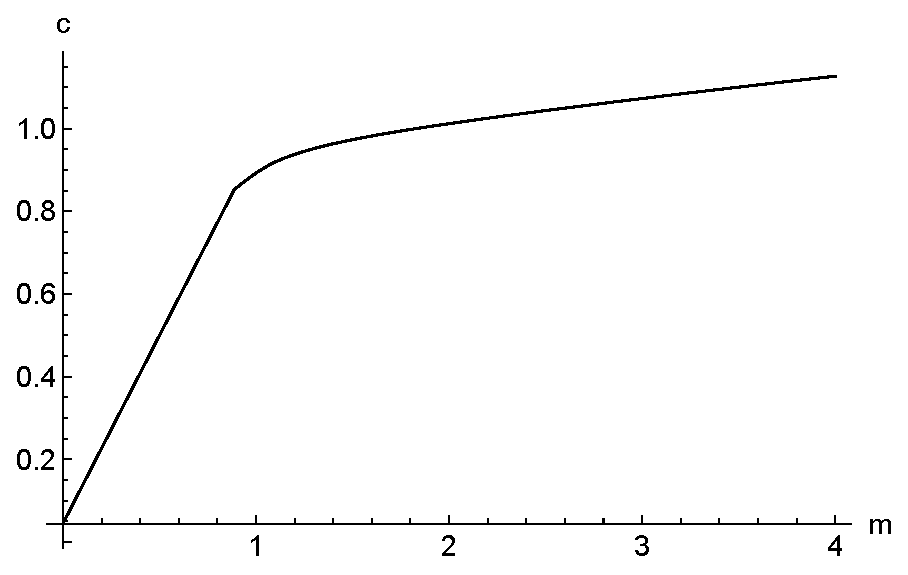
\includegraphics[width=6in]{./Figures/PlotctMultContr}
  \caption{$\cFunc({m}_{1})$ With Portfolio Choice}
  \label{fig:PlotctMultContr}
\end{figure}

\hypertarget{PlotRiskySharetOfat}{}
\begin{figure}
  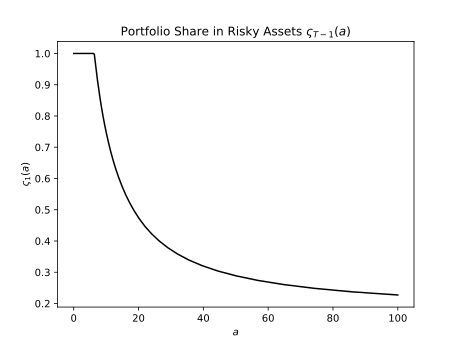
\includegraphics[width=6in]{./Figures/PlotRiskySharetOfat}
  \caption{Portfolio Share in Risky Assets in First Period $\Shr({a})$}
  \label{fig:PlotRiskySharetOfat}
\end{figure}
\end{document}
